% E1 report for the supervisors. Built with `python paper/build.py --report e1` (paper/README.md).
% Content: a translation of paper/sections/e1_notes_fr.md (the author's notes), in their order; the zone-type
% definitions come from paper/sections/e3_notes_fr.md. Where the notes and the repository disagreed on a fact listed in
% the Phase 0 review, the repository's version is written. Every number is a macro of ../numbers.tex, or is written as it
% is with a source comment and the num-ok marker.
\documentclass[10pt]{article}

\usepackage[T1]{fontenc}
\usepackage{lmodern}
\usepackage{amsmath}
\usepackage{amssymb}
\usepackage{graphicx}
\usepackage{booktabs}
\usepackage[numbers]{natbib}
\usepackage[textsize=scriptsize]{todonotes}
\setlength{\marginparwidth}{2.6cm}
\usepackage{hyperref}

\graphicspath{{../figures/out/}}

% Notation macros. One macro per symbol; the comment gives its name in the
% code (src/helplessness, experiments/E2_online_4zones/twin.py).
% Every macro is wrapped in \ensuremath, so it works in and out of math mode.

% Controllability I(a;s'|s), measures.controllability.controllability_from_tensor.
\newcommand{\MI}[3]{\ensuremath{I(#1;#2\mid #3)}}
% I_hat: controllability of the belief T_hat.
\newcommand{\Ihat}{\ensuremath{\hat{I}}}
% I_ref: controllability of the count-matched reference (not the analytic value).
\newcommand{\Iref}{\ensuremath{\hat{I}_{\mathrm{ref}}}}
% I_star: controllability of the true kernel P.
\newcommand{\Istar}{\ensuremath{I^{*}}}
% b = I_hat - I_ref.
\newcommand{\bhat}{\ensuremath{\hat{b}}}
% Believed transition kernel.
\newcommand{\That}{\ensuremath{\hat{T}}}
% True transition kernel.
\newcommand{\Ptrue}{\ensuremath{P}}
% Reference-environment kernel.
\newcommand{\Pref}{\ensuremath{P_{\mathrm{ref}}}}
% delta = V_star - V^{pi_hat}, the belief's policy evaluated under P.
\newcommand{\regret}{\ensuremath{\Delta}}
% l1: per-pair L1 error between T_hat and P.
\newcommand{\Lone}{\ensuremath{L_{1}}}
% Optimal value under P.
\newcommand{\Vstar}{\ensuremath{V^{*}}}
% Value under P of the policy derived from T_hat.
\newcommand{\Vpihat}{\ensuremath{V^{\hat{\pi}}}}
% Base-2 logarithm (written as a macro: its 2 is notation, not a number).
\newcommand{\logtwo}{\log_{2}}
% The null hypothesis of a test (written as a macro: its 0 is notation, not a number).
\newcommand{\Hnull}{\ensuremath{H_{0}}}
% R: the reward on arrival at the goal (E1's calibrated parameter).
\newcommand{\Rgoal}{\ensuremath{R}}
% Visit counts N(s,a).
\newcommand{\counts}{\ensuremath{N}}
% Paired online - matched difference of a quantity, e.g. \gap{\bhat}.
\newcommand{\gap}[1]{\ensuremath{#1^{\mathrm{on}} - #1^{\mathrm{m}}}}

% Reserved for E3.
% I_s: controllability of the decoded s-space kernel (E3 main measure).
\newcommand{\Is}{\ensuremath{\hat{I}_{s}}}
% I_z: controllability in latent space (E3 secondary measure).
\newcommand{\Iz}{\ensuremath{\hat{I}_{z}}}

% --- E3 (world model) ---------------------------------------------------------
% The name of E3's offline calibration condition (written as a macro: its 0 is a name, not a number).
% Robust: \nobreakdash breaks in moving arguments (captions, section titles).
\DeclareRobustCommand{\EThreeZero}{E3\nobreakdash-0}
% h_0: the RSSM's learned initial deterministic state (the canonical probe's context).
\newcommand{\hzero}{\ensuremath{h_{0}}}
% I_s projected on the 5 reachable successors (secondary measure).
\newcommand{\Isproj}{\ensuremath{\hat{I}_{s}^{\mathrm{proj}}}}
% alpha_app: position / appearance index of diagnostic D1.
\newcommand{\alphaapp}{\ensuremath{\alpha_{\mathrm{app}}}}
% alpha: weight of an action-independent component in the predicted kernel
% (campaign analysis; distinct from alpha_app and from E2's Dirichlet alpha).
\newcommand{\alphaind}{\ensuremath{\alpha}}
% K_s: decoded prior draws per (s, a) for the s-space kernel.
\newcommand{\Ks}{\ensuremath{K_{s}}}
% L1 errors of criterion C-b: world model and tabular twin, against P.
\newcommand{\LoneWM}{\ensuremath{L_{1}^{\mathrm{WM}}}}
\newcommand{\LoneB}{\ensuremath{L_{1}^{B}}}
% Off-support mass of a predicted kernel.
\newcommand{\offmass}{\ensuremath{m_{\mathrm{off}}}}
% p_goal: the goal head's probability that a latent state is the goal.
\newcommand{\pgoal}{\ensuremath{p_{\mathrm{goal}}}}
% KL weights: beta_dyn trains the prior only, beta_rep pulls the posterior.
\newcommand{\betadyn}{\ensuremath{\beta_{\mathrm{dyn}}}}
\newcommand{\betarep}{\ensuremath{\beta_{\mathrm{rep}}}}
% Jensen-Shannon divergence.
\newcommand{\JS}{\ensuremath{\mathrm{JS}}}
% The critic's value estimate.
\newcommand{\Vhat}{\ensuremath{\hat{V}}}
% The tabular twin (condition B).
\newcommand{\twin}{\ensuremath{B}}
% Names of the calibration criteria and diagnostics.
\DeclareRobustCommand{\Ca}{C\nobreakdash-a}
\DeclareRobustCommand{\Cb}{C\nobreakdash-b}
\DeclareRobustCommand{\Cc}{C\nobreakdash-c}
\newcommand{\DOne}{D1}
\newcommand{\DTwo}{D2}

% --- Pending values ------------------------------------------------------------
% A number or figure that depends on a batch not run yet (the E3 final campaign).
% Its argument (the macro or figure name) is not shown; numbers.tex writes it.
\newcommand{\pending}[1]{\textcolor{orange}{\textbf{[pending]}}}

% Generated by paper/numbers/gen_numbers.py -- never edit by hand.
% Generated by paper/numbers/gen_numbers.py -- do not edit by hand.
% Rerun `python paper/build.py --numbers` after any change to the results.

% src: experiments/E2_online_4zones/artifacts/figures/csv/F2_null_model_paired_diff.csv :: n_seeds (constant over rows quantity=b, zone=controllable_noisy)
\newcommand{\eTwoNSeeds}{20}
% src: experiments/E2_online_4zones/artifacts/figures/csv/F2_null_model_paired_diff.csv :: number of distinct checkpoint values (quantity=b, zone=controllable_noisy)
\newcommand{\eTwoNCheckpoints}{16}
% src: experiments/E2_online_4zones/artifacts/figures/csv/table3_budget_trend_power_law.csv :: n_points (quantity=b, zone=controllable_noisy)
\newcommand{\eTwoGapFitNPoints}{11}
% src: experiments/E2_online_4zones/artifacts/figures/csv/table3_budget_trend_power_law.csv :: exponent (quantity=b, zone=controllable_noisy)
\newcommand{\eTwoGapExponent}{\ensuremath{+0.005}}
% src: experiments/E2_online_4zones/artifacts/figures/csv/table3_budget_trend_power_law.csv :: exponent_bootstrap_ci95_low (quantity=b, zone=controllable_noisy)
\newcommand{\eTwoGapExponentCILow}{\ensuremath{-0.210}}
% src: experiments/E2_online_4zones/artifacts/figures/csv/table3_budget_trend_power_law.csv :: exponent_bootstrap_ci95_high (quantity=b, zone=controllable_noisy)
\newcommand{\eTwoGapExponentCIHigh}{\ensuremath{+0.274}}
% src: experiments/E2_online_4zones/artifacts/figures/csv/table1_paired_diff_by_zone.csv :: mean_diff (checkpoint=100000, zone=controllable_noisy, quantity=b): E2's online - matched gap on b in the CN zone, the effect E1 and E3 refer to
\newcommand{\eTwoEffectCN}{\ensuremath{-0.02}}
% src: configs/zones/e1_4zones.yaml :: grid_shape (square)
\newcommand{\eThreeGridSize}{12}
% src: configs/zones/e1_4zones.yaml :: blocks.*.rows / cols (side of every block)
\newcommand{\eThreeZoneSize}{5}
% src: configs/zones/e1_4zones.yaml :: number of blocks
\newcommand{\eThreeNZones}{4}
% src: src/helplessness/envs/dynamics/__init__.py :: N_ACTIONS
\newcommand{\eThreeNActions}{5}
% src: configs/zones/e1_4zones.yaml :: blocks.ne.p = blocks.se.p
\newcommand{\eThreeNoiseP}{0.125}
% src: configs/zones/e1_4zones.yaml :: 1 - p + p / N_ACTIONS (blocks.ne.p; envs/dynamics)
\newcommand{\eThreeNoiseMain}{0.9}
% src: configs/zones/e1_4zones.yaml :: p / N_ACTIONS (blocks.ne.p; envs/dynamics)
\newcommand{\eThreeNoiseMinor}{0.025}
% src: experiments/E3_worldmodel_4zones/config.yaml :: episode.goal_reward
\newcommand{\eThreeGoalReward}{\ensuremath{+50}}
% src: experiments/E3_worldmodel_4zones/config.yaml :: episode.step_reward
\newcommand{\eThreeStepReward}{\ensuremath{-1}}
% src: experiments/E3_worldmodel_4zones/config.yaml :: episode.max_steps
\newcommand{\eThreeEpisodeHorizon}{36}
% src: experiments/E3_worldmodel_4zones/config.yaml :: episode.gamma
\newcommand{\eThreeGamma}{0.9}
% src: experiments/E3_worldmodel_4zones/config.yaml :: episode.step_reward / (1 - episode.gamma)
\newcommand{\eThreeVNoGoal}{\ensuremath{-10}}
% src: configs/e3/gpu_campaign.yaml :: render.k
\newcommand{\eThreeRenderScale}{6}
% src: configs/e3/gpu_campaign.yaml :: render.cielab_marker_min_dist
\newcommand{\eThreeMarkerMinDist}{30}
% src: configs/e3/gpu_campaign.yaml :: model.n_vars
\newcommand{\eThreeLatentVars}{8}
% src: configs/e3/gpu_campaign.yaml :: model.n_classes
\newcommand{\eThreeLatentClasses}{8}
% src: configs/e3/gpu_campaign.yaml :: train.free_bits
\newcommand{\eThreeFreeBits}{0}
% src: configs/e3/gpu_campaign.yaml :: train.lr
\newcommand{\eThreeLr}{\ensuremath{10^{-3}}}
% src: configs/e3/gpu_campaign.yaml :: train.lr_after_switch
\newcommand{\eThreeLrAfterSwitch}{\ensuremath{10^{-4}}}
% src: configs/e3/gpu_campaign.yaml :: train.latent_estimator.switch_n_pairs
\newcommand{\eThreeSwitchPairs}{64}
% src: configs/e3/gpu_campaign.yaml :: train.latent_estimator.switch_eval_every
\newcommand{\eThreeSwitchEvalEvery}{50}
% src: configs/e3/gpu_campaign.yaml :: train.latent_estimator.switch_js_threshold
\newcommand{\eThreeSwitchJS}{3}
% src: configs/e3/gpu_campaign.yaml :: train.latent_estimator.switch_consecutive
\newcommand{\eThreeSwitchConsecutive}{5}
% src: configs/e3/gpu_campaign.yaml :: train.latent_estimator.collapse_js_threshold
\newcommand{\eThreeCollapseJS}{1}
% src: configs/e3/gpu_campaign.yaml :: train.batch_size
\newcommand{\eThreeBatchWindows}{16}
% src: configs/e3/gpu_campaign.yaml :: train.seq_len
\newcommand{\eThreeWindowLength}{64}
% src: configs/e3/gpu_e30b_win64.yaml :: train.batch_size x train.seq_len
\newcommand{\eThreeFramesPerUpdate}{1024}
% src: configs/e3/gpu_e30b_win16.yaml :: train.batch_size
\newcommand{\eThreeShortBatchWindows}{64}
% src: configs/e3/gpu_e30b_win16.yaml :: train.seq_len
\newcommand{\eThreeShortWindowLength}{16}
% src: configs/e3/gpu_campaign.yaml :: train.replay_ratio
\newcommand{\eThreeReplayRatio}{0.6}
% src: configs/e3/agent_mini.yaml :: train.replay_ratio
\newcommand{\eThreeReplayRatioMini}{2}
% src: configs/e3/gpu_campaign.yaml :: agent.epsilon
\newcommand{\eThreeEpsilon}{0.1}
% src: configs/e3/gpu_e30.yaml :: collection.epsilon
\newcommand{\eThreeEpsilonOffline}{1}
% src: configs/e3/gpu_campaign.yaml :: agent.k_act
\newcommand{\eThreeKAct}{16}
% src: configs/e3/gpu_campaign.yaml :: agent.horizon
\newcommand{\eThreeImagHorizon}{15}
% src: results/E3_worldmodel_4zones/*gpu_pilot_closed_loop__seed{00,05}*/meta.yaml :: agent.tie_tol_abs (the 4 runs agree)
\newcommand{\eThreeTieTol}{0.0751}
% src: configs/e3/gpu_campaign.yaml :: measure.kernel_k_s (= real_context.kernel_draws; checked against measures.kernel_probe.draws_for_l1_floor(CN kernel, 0.02))
\newcommand{\eThreeKs}{1358}
% src: results/E3_worldmodel_4zones/*gpu_e30b_win64__seed00* (experimental) arrays.npz P_true :: max over the CN rows of measures.kernel_probe.expected_l1_sampling_floor(row, 32)
\newcommand{\eThreeFloorOldK}{0.13}
% src: configs/e3/gpu_campaign.yaml :: measure.real_context.burn_in
\newcommand{\eThreeContextBurnIn}{8}
% src: configs/e3/gpu_pilot_closed_loop.yaml :: measure.real_context.max_per_state
\newcommand{\eThreeContextsPilot}{50}
% src: configs/e3/gpu_campaign.yaml :: measure.real_context.max_per_state
\newcommand{\eThreeContextsFinal}{200}
% src: configs/e3/gpu_campaign.yaml :: measure.iz_mc_samples_training
\newcommand{\eThreeIzMcTraining}{2000}
% src: configs/e3/gpu_campaign.yaml :: measure.iz_mc_samples_final
\newcommand{\eThreeIzMcFinal}{4096}
% src: configs/e3/gpu_pilot_closed_loop.yaml :: measure.checkpoint_goal_kernel.draws
\newcommand{\eThreeGoalDrawsPilot}{256}
% src: configs/e3/gpu_campaign.yaml :: measure.checkpoint_goal_kernel.goal_draws
\newcommand{\eThreeGoalDraws}{10{,}000}
% src: configs/e3/gpu_e30.yaml :: seeds[0]
\newcommand{\eThreeZeroSeedA}{0}
% src: configs/e3/gpu_e30.yaml :: seeds[1]
\newcommand{\eThreeZeroSeedB}{5}
% src: configs/e3/gpu_e30.yaml :: budget.total_steps + budget.prefill_steps
\newcommand{\eThreeZeroEnvSteps}{100{,}000}
% src: configs/e3/gpu_e30.yaml :: (budget.total_steps + budget.prefill_steps) x train.replay_ratio
\newcommand{\eThreeZeroGradSteps}{60{,}000}
% src: configs/e3/gpu_campaign.yaml :: budget.total_steps + budget.prefill_steps
\newcommand{\eThreeBudget}{300{,}000}
% src: configs/e3/gpu_pilot_closed_loop.yaml :: budget.total_steps + budget.prefill_steps
\newcommand{\eThreePilotBudget}{300{,}000}
% src: configs/e3/gpu_pilot_closed_loop.yaml :: seeds[0]
\newcommand{\eThreePilotSeedA}{0}
% src: configs/e3/gpu_pilot_closed_loop.yaml :: seeds[1]
\newcommand{\eThreePilotSeedB}{5}
% src: configs/e3/gpu_campaign.yaml :: seeds[0]
\newcommand{\eThreeCampaignSeedA}{1}
% src: configs/e3/gpu_campaign.yaml :: seeds[1]
\newcommand{\eThreeCampaignSeedB}{6}
% src: results/E3_worldmodel_4zones/*gpu_e30b_win{64,16}__seed{00,05}*/arrays.npz P_true :: CN zone mean of controllability_per_state
\newcommand{\eThreeTrueICN}{1.65}
% src: results/E3_worldmodel_4zones/*gpu_e30b_win{64,16}__seed{00,05}*/arrays.npz P_true :: CD zone mean of controllability_per_state
\newcommand{\eThreeTrueICD}{2.32}
% src: results/E3_worldmodel_4zones/*gpu_e30b_win{64,16}__seed{00,05}*/arrays.npz P_true :: UD zone mean of controllability_per_state, env - ref
\newcommand{\eThreeTrueBUD}{\ensuremath{-2.32}}
% src: results/E3_worldmodel_4zones/*gpu_e30b_win{64,16}__seed{00,05}*/results.json :: min of I_s_by_category_real.controllable_noisy (8 runs)
\newcommand{\eThreeZeroIsCNMin}{1.93}
% src: results/E3_worldmodel_4zones/*gpu_e30b_win{64,16}__seed{00,05}*/results.json :: max of I_s_by_category_real.controllable_noisy (8 runs)
\newcommand{\eThreeZeroIsCNMax}{1.95}
% src: results/E3_worldmodel_4zones/*gpu_e30b_win{64,16}__seed{00,05}*/results.json :: min of h_only_probe.test_accuracy (8 runs)
\newcommand{\eThreeZeroProbeHMin}{0.905}
% src: results/E3_worldmodel_4zones/*gpu_e30b_win{64,16}__seed{00,05}*/results.json :: max of h_only_probe.test_accuracy (8 runs)
\newcommand{\eThreeZeroProbeHMax}{0.917}
% src: results/E3_worldmodel_4zones/*gpu_e30b_win{64,16}__seed{00,05}*/results.json :: min of z_only_probe.test_accuracy (8 runs)
\newcommand{\eThreeZeroProbeZMin}{0.993}
% src: results/E3_worldmodel_4zones/*gpu_e30b_win{64,16}__seed{00,05}*/results.json :: max of z_only_probe.test_accuracy (8 runs)
\newcommand{\eThreeZeroProbeZMax}{0.999}
% src: results/E3_worldmodel_4zones/*gpu_e30b_win{64,16}__seed{00,05}*/ :: min over the 4 pairs of aggregate_b b(I_s), UD
\newcommand{\eThreeZeroFloorUDMin}{\ensuremath{-2.27}}
% src: results/E3_worldmodel_4zones/*gpu_e30b_win{64,16}__seed{00,05}*/ :: max over the 4 pairs of aggregate_b b(I_s), UD
\newcommand{\eThreeZeroFloorUDMax}{\ensuremath{-2.19}}
% src: results/E3_worldmodel_4zones/*gpu_e30b_win{64,16}__seed{00,05}*/ :: min over the 4 pairs of aggregate_b b(I_s), CN and CD
\newcommand{\eThreeZeroFloorCtrlMin}{\ensuremath{-0.013}}
% src: results/E3_worldmodel_4zones/*gpu_e30b_win{64,16}__seed{00,05}*/ :: max over the 4 pairs of aggregate_b b(I_s), CN and CD
\newcommand{\eThreeZeroFloorCtrlMax}{\ensuremath{+0.008}}
% src: results/E3_worldmodel_4zones/*gpu_e30b_win{64,16}__seed{00,05}*/results.json :: min of real_context.frequent_outcome.controllable_noisy (8 runs)
\newcommand{\eThreeTFourCNMin}{0.89}
% src: results/E3_worldmodel_4zones/*gpu_e30b_win{64,16}__seed{00,05}*/results.json :: max of real_context.frequent_outcome.controllable_noisy (8 runs)
\newcommand{\eThreeTFourCNMax}{0.91}
% src: results/E3_worldmodel_4zones/*gpu_e30b_win{64,16}__seed{00,05}*/results.json :: min of real_context.frequent_outcome.uncontrollable_noisy (4 env runs)
\newcommand{\eThreeTFourUNMin}{0.69}
% src: results/E3_worldmodel_4zones/*gpu_e30b_win{64,16}__seed{00,05}*/results.json :: max of real_context.frequent_outcome.uncontrollable_noisy (4 env runs)
\newcommand{\eThreeTFourUNMax}{0.77}
% src: results/E3_worldmodel_4zones/*gpu_e30_bridge*/recomputed/final__ks1358__20260930T124347Z/results.json :: d2_boundary_mean
\newcommand{\eThreeBridgeDTwoBoundary}{4.3}
% src: results/E3_worldmodel_4zones/*gpu_e30_bridge*/recomputed/final__ks1358__20260930T124347Z/results.json :: d2_within_zone_mean
\newcommand{\eThreeBridgeDTwoWithin}{2.9}
% src: results/E3_worldmodel_4zones/theme_sensitivity/draw_NN.json :: min of switch_step (10 draws)
\newcommand{\eThreeThemeSwitchMin}{2051}
% src: results/E3_worldmodel_4zones/theme_sensitivity/draw_NN.json :: max of switch_step (10 draws)
\newcommand{\eThreeThemeSwitchMax}{6401}
% src: results/E3_worldmodel_4zones/theme_sensitivity/*.json :: number of records
\newcommand{\eThreeThemeRuns}{16}
% src: results/E3_worldmodel_4zones/theme_sensitivity/*.json :: records with status separation_not_reached
\newcommand{\eThreeThemeCensored}{1}
% src: reports/diagnostics_grid12x12__4zones__pair-experimental__worldmodel-agent-agent_mini__seed00__20260930T193212Z/diagnostics.json :: a.goal_frames_total_at_resume_point
\newcommand{\eThreeMiniGoalFrames}{13}
% src: reports/diagnostics_grid12x12__4zones__pair-experimental__worldmodel-agent-agent_mini__seed00__20260930T193212Z/diagnostics.json :: a.rows[first].P_batch_without_positive (the switch)
\newcommand{\eThreeMiniNoGoalAtSwitch}{81}
% src: reports/diagnostics_grid12x12__4zones__pair-experimental__worldmodel-agent-agent_mini__seed00__20260930T193212Z/diagnostics.json :: a.rows[last].P_batch_without_positive (18,000)
\newcommand{\eThreeMiniNoGoalAtResume}{91}
% src: reports/gradients_vs_data_grid12x12__4zones__pair-experimental__worldmodel-agent-agent_mini__seed00__20260930T193212Z/result.json :: criterion.start
\newcommand{\eThreeMiniMassStart}{0.28}
% src: reports/gradients_vs_data_grid12x12__4zones__pair-experimental__worldmodel-agent-agent_mini__seed00__20260930T193212Z/result.json :: criterion.end
\newcommand{\eThreeMiniMassEnd}{0.49}
% src: reports/gradients_vs_data_grid12x12__4zones__pair-experimental__worldmodel-agent-agent_mini__seed00__20260930T193212Z/result.json :: steps_done
\newcommand{\eThreeMiniExtraGradSteps}{20{,}000}
% src: results/E3_worldmodel_4zones/*gpu_pilot_closed_loop__seed{00,05}*/checkpoints.jsonl :: min over the 4 runs of the last record's goal_diagnostics.median_mass_on_goal_pairs
\newcommand{\eThreePilotGoalMassFinal}{1.00}
% src: results/E3_worldmodel_4zones/*gpu_pilot_closed_loop__seed{00,05}*/checkpoints.jsonl :: min over the 4 runs of the last record's success_rate (last 100 episodes)
\newcommand{\eThreePilotSuccessFinal}{1.00}
% src: results/E3_worldmodel_4zones/*gpu_pilot_closed_loop__seed{00,05}*/checkpoints.jsonl :: min over runs and zones of the last record's agent_delta.real_contexts.delta_by_zone
\newcommand{\eThreePilotDeltaMin}{0.00}
% src: results/E3_worldmodel_4zones/*gpu_pilot_closed_loop__seed{00,05}*/checkpoints.jsonl :: max over runs and zones of the last record's agent_delta.real_contexts.delta_by_zone
\newcommand{\eThreePilotDeltaMax}{0.75}
% src: results/E3_worldmodel_4zones/gpu_campaign/ (campaign_analysis.analyse main pairs; aggregate_b.mean_ci95) :: b(I_s) at the budget, UD, mean  [PENDING: the final campaign]
\newcommand{\eThreeCampaignBUDMean}{\pending{eThreeCampaignBUDMean}}
% src: results/E3_worldmodel_4zones/gpu_campaign/ (campaign_analysis.analyse main pairs; aggregate_b.mean_ci95) :: b(I_s) at the budget, UD, low  [PENDING: the final campaign]
\newcommand{\eThreeCampaignBUDLow}{\pending{eThreeCampaignBUDLow}}
% src: results/E3_worldmodel_4zones/gpu_campaign/ (campaign_analysis.analyse main pairs; aggregate_b.mean_ci95) :: b(I_s) at the budget, UD, high  [PENDING: the final campaign]
\newcommand{\eThreeCampaignBUDHigh}{\pending{eThreeCampaignBUDHigh}}
% src: results/E3_worldmodel_4zones/gpu_campaign/ (campaign_analysis.analyse main pairs; aggregate_b.mean_ci95) :: b(I_s) at the budget, CN, mean  [PENDING: the final campaign]
\newcommand{\eThreeCampaignBCNMean}{\pending{eThreeCampaignBCNMean}}
% src: results/E3_worldmodel_4zones/gpu_campaign/ (campaign_analysis.analyse main pairs; aggregate_b.mean_ci95) :: b(I_s) at the budget, CN, low  [PENDING: the final campaign]
\newcommand{\eThreeCampaignBCNLow}{\pending{eThreeCampaignBCNLow}}
% src: results/E3_worldmodel_4zones/gpu_campaign/ (campaign_analysis.analyse main pairs; aggregate_b.mean_ci95) :: b(I_s) at the budget, CN, high  [PENDING: the final campaign]
\newcommand{\eThreeCampaignBCNHigh}{\pending{eThreeCampaignBCNHigh}}
% src: results/E3_worldmodel_4zones/gpu_campaign/ (campaign_analysis.analyse main pairs; aggregate_b.mean_ci95) :: b(I_s) at the budget, UN, mean  [PENDING: the final campaign]
\newcommand{\eThreeCampaignBUNMean}{\pending{eThreeCampaignBUNMean}}
% src: results/E3_worldmodel_4zones/gpu_campaign/ (campaign_analysis.analyse main pairs; aggregate_b.mean_ci95) :: b(I_s) at the budget, UN, low  [PENDING: the final campaign]
\newcommand{\eThreeCampaignBUNLow}{\pending{eThreeCampaignBUNLow}}
% src: results/E3_worldmodel_4zones/gpu_campaign/ (campaign_analysis.analyse main pairs; aggregate_b.mean_ci95) :: b(I_s) at the budget, UN, high  [PENDING: the final campaign]
\newcommand{\eThreeCampaignBUNHigh}{\pending{eThreeCampaignBUNHigh}}
% src: results/E3_worldmodel_4zones/gpu_campaign/ (campaign_analysis.analyse main pairs; aggregate_b.mean_ci95) :: b(I_s) at the budget, CD, mean  [PENDING: the final campaign]
\newcommand{\eThreeCampaignBCDMean}{\pending{eThreeCampaignBCDMean}}
% src: results/E3_worldmodel_4zones/gpu_campaign/ (campaign_analysis.analyse main pairs; aggregate_b.mean_ci95) :: b(I_s) at the budget, CD, low  [PENDING: the final campaign]
\newcommand{\eThreeCampaignBCDLow}{\pending{eThreeCampaignBCDLow}}
% src: results/E3_worldmodel_4zones/gpu_campaign/ (campaign_analysis.analyse main pairs; aggregate_b.mean_ci95) :: b(I_s) at the budget, CD, high  [PENDING: the final campaign]
\newcommand{\eThreeCampaignBCDHigh}{\pending{eThreeCampaignBCDHigh}}
% src: configs/zones/e1_4zones.yaml :: grid_shape (square)
\newcommand{\eOneGridSize}{12}
% src: configs/zones/e1_4zones.yaml :: blocks.*.rows / cols (side of every block)
\newcommand{\eOneZoneSize}{5}
% src: configs/zones/e1_4zones.yaml :: number of blocks
\newcommand{\eOneNZones}{4}
% src: configs/zones/e1_4zones.yaml :: corridor cells of experiments/E1_offline_4zones/env.py::build_layout
\newcommand{\eOneCorridorCells}{44}
% src: configs/zones/e1_4zones.yaml :: cells of a block (env.py::build_layout)
\newcommand{\eOneZoneCells}{25}
% src: configs/zones/e1_4zones.yaml :: interior cells of a block (envs.zones.interior_mask)
\newcommand{\eOneInteriorCells}{9}
% src: src/helplessness/envs/dynamics/__init__.py :: N_ACTIONS
\newcommand{\eOneNActions}{5}
% src: configs/zones/e1_4zones.yaml :: blocks.ne.p = blocks.se.p
\newcommand{\eOneNoiseP}{0.125}
% src: configs/zones/e1_4zones.yaml :: 1 - p + p / N_ACTIONS
\newcommand{\eOneNoiseMain}{0.9}
% src: configs/zones/e1_4zones.yaml :: p / N_ACTIONS
\newcommand{\eOneNoiseMinor}{0.025}
% src: experiments/E1_offline_4zones/config.yaml :: gamma
\newcommand{\eOneGamma}{0.9}
% src: experiments/E1_offline_4zones/config.yaml :: goal_reward
\newcommand{\eOneGoalReward}{50}
% src: experiments/E1_offline_4zones/config.yaml :: step_reward
\newcommand{\eOneStepReward}{\ensuremath{-1}}
% src: experiments/E1_offline_4zones/config.yaml :: 1 / (1 - gamma)
\newcommand{\eOneStepCostHorizon}{10}
% src: experiments/E1_offline_4zones/config.yaml :: (1 / (1 - gamma)) / goal_reward
\newcommand{\eOneStepCostShare}{20}
% src: experiments/E1_offline_4zones/artifacts/calibration_report.csv :: number of rows
\newcommand{\eOneCalibCombos}{36}
% src: experiments/E1_offline_4zones/artifacts/calibration_report.csv :: distinct gamma
\newcommand{\eOneCalibGammas}{6}
% src: experiments/E1_offline_4zones/artifacts/calibration_report.csv :: distinct R
\newcommand{\eOneCalibRewards}{3}
% src: experiments/E1_offline_4zones/artifacts/calibration_report.csv :: distinct direction
\newcommand{\eOneCalibDirections}{2}
% src: experiments/E1_offline_4zones/artifacts/calibration_report.csv :: rows per direction (equal for both)
\newcommand{\eOneCalibPerDirection}{18}
% src: experiments/E1_offline_4zones/artifacts/calibration_report.csv :: max exterior_max_abs_diff_exp_vs_ctrl (checked against recommendation.txt)
\newcommand{\eOneExteriorDiffCtrl}{\ensuremath{3.55 \times 10^{-11}}}
% src: experiments/E1_offline_4zones/artifacts/calibration_report.csv :: max exterior_max_abs_diff_away_vs_toward (checked against recommendation.txt)
\newcommand{\eOneExteriorDiffDirection}{\ensuremath{1.45 \times 10^{-11}}}
% src: experiments/E1_offline_4zones/artifacts/calibration_report.csv :: max |interior_gap_nw|, |interior_gap_se| (checked against recommendation.txt)
\newcommand{\eOneInteriorGapMax}{30.66}
% src: experiments/E1_offline_4zones/artifacts/calibration_report.csv :: away_from_goal rows with well_shape_nw = well_shape_se = well
\newcommand{\eOneAwayWells}{18}
% src: experiments/E1_offline_4zones/artifacts/calibration_report.csv :: toward_goal rows with well_shape_nw = negligible
\newcommand{\eOneTowardNegligible}{18}
% src: experiments/E1_offline_4zones/artifacts/gradient_curves.csv :: max |V_mean(NW) - V_mean(SE)|, same env, over the whole sweep
\newcommand{\eOneProfileDiffNWSE}{\ensuremath{1.4 \times 10^{-14}}}
% src: experiments/E1_offline_4zones/artifacts/measurements.csv :: distinct seed
\newcommand{\eOneNSeeds}{20}
% src: experiments/E1_offline_4zones/artifacts/measurements.csv :: number of rows
\newcommand{\eOneNRows}{2400}
% src: experiments/E1_offline_4zones/artifacts/measurements.csv :: rows with delta < 0
\newcommand{\eOneDeltaViolations}{0}
% src: experiments/E1_offline_4zones/artifacts/measurements.csv :: b, UD, n = 1000, mean over seeds (e1_sources.step_b: report.py's filters and functions; checked against etape_b_report.txt)
\newcommand{\eOneBUDMean}{\ensuremath{-2.32193}}
% src: experiments/E1_offline_4zones/artifacts/measurements.csv :: b, UD, n = 1000, sd over seeds (e1_sources.step_b: report.py's filters and functions; checked against etape_b_report.txt)
\newcommand{\eOneBUDSd}{0}
% src: experiments/E1_offline_4zones/artifacts/measurements.csv :: b, UN, n = 1000, mean over seeds (e1_sources.step_b: report.py's filters and functions; checked against etape_b_report.txt)
\newcommand{\eOneBUNMean}{\ensuremath{-1.6518}}
% src: experiments/E1_offline_4zones/artifacts/measurements.csv :: b, UN, n = 1000, sd over seeds (e1_sources.step_b: report.py's filters and functions; checked against etape_b_report.txt)
\newcommand{\eOneBUNSd}{0.0056}
% src: experiments/E1_offline_4zones/artifacts/measurements.csv :: |mean b - predicted b|, UN, n = 1000 (e1_sources.step_b: report.py's filters and functions; checked against etape_b_report.txt)
\newcommand{\eOneBUNError}{0.0011}
% src: experiments/E1_offline_4zones/artifacts/measurements.csv :: b, CN, n = 1000, mean over seeds (e1_sources.step_b: report.py's filters and functions; checked against etape_b_report.txt)
\newcommand{\eOneBCNMean}{\ensuremath{-0.0003}}
% src: experiments/E1_offline_4zones/artifacts/measurements.csv :: b, CN, n = 1000, sd over seeds (e1_sources.step_b: report.py's filters and functions; checked against etape_b_report.txt)
\newcommand{\eOneBCNSd}{0.0064}
% src: experiments/E1_offline_4zones/artifacts/measurements.csv :: b, CD, n = 1000, mean over seeds (e1_sources.step_b: report.py's filters and functions; checked against etape_b_report.txt)
\newcommand{\eOneBCDMean}{0}
% src: experiments/E1_offline_4zones/report.py :: predicted_b(uncontrollable_noisy)
\newcommand{\eOnePredBUN}{\ensuremath{-1.6529}}
% src: experiments/E1_offline_4zones/report.py :: predicted_b(uncontrollable_noisy)
\newcommand{\eOnePredBUNShort}{\ensuremath{-1.65}}
% src: experiments/E1_offline_4zones/report.py :: predicted_b(uncontrollable_deterministic)
\newcommand{\eOnePredBUD}{\ensuremath{-2.32}}
% src: experiments/E1_offline_4zones/artifacts/measurements.csv :: I_hat - I_star, UN, n = 10, env (e1_sources.step_b: report.py's filters and functions; checked against etape_b_report.txt)
\newcommand{\eOneBiasIhat}{\ensuremath{+0.163}}
% src: experiments/E1_offline_4zones/artifacts/measurements.csv :: I_hat - I_star, UN, n = 10, control (e1_sources.step_b: report.py's filters and functions; checked against etape_b_report.txt)
\newcommand{\eOneBiasIref}{\ensuremath{+0.202}}
% src: experiments/E1_offline_4zones/artifacts/measurements.csv :: |b - predicted b|, UN, n = 10 (e1_sources.step_b: report.py's filters and functions; checked against etape_b_report.txt)
\newcommand{\eOneBiasResidual}{0.0395}
% src: experiments/E1_offline_4zones/artifacts/measurements.csv :: cancellation factor (report.py bias_cancellation_factor), UN, n = 10 (e1_sources.step_b: report.py's filters and functions; checked against etape_b_report.txt)
\newcommand{\eOneBiasFactor}{4.6}
% src: experiments/E1_offline_4zones/artifacts/measurements.csv :: delta, CN, interior, env, n = 10, mean over seeds (e1_sources.step_b: report.py's filters and functions; checked against etape_b_report.txt)
\newcommand{\eOneDeltaCNTen}{0.43}
% src: experiments/E1_offline_4zones/artifacts/measurements.csv :: delta, CN, interior, env, n = 30, mean over seeds (e1_sources.step_b: report.py's filters and functions; checked against etape_b_report.txt)
\newcommand{\eOneDeltaCNThirty}{0.36}
% src: experiments/E1_offline_4zones/artifacts/measurements.csv :: delta, CN, interior, env, n = 100, mean over seeds (e1_sources.step_b: report.py's filters and functions; checked against etape_b_report.txt)
\newcommand{\eOneDeltaCNHundred}{0.095}
% src: experiments/E1_offline_4zones/artifacts/measurements.csv :: delta, CN, interior, env, n = 300, mean over seeds (e1_sources.step_b: report.py's filters and functions; checked against etape_b_report.txt)
\newcommand{\eOneDeltaCNThreeHundred}{0.007}
% src: experiments/E1_offline_4zones/artifacts/measurements.csv :: delta, CN, interior, env, n = 1000, mean over seeds (e1_sources.step_b: report.py's filters and functions; checked against etape_b_report.txt)
\newcommand{\eOneDeltaCNThousand}{0}
% src: experiments/E1_offline_4zones/artifacts/measurements.csv :: l1, CN, whole zone, n = 10 (e1_sources.step_b: report.py's filters and functions; checked against etape_b_report.txt)
\newcommand{\eOneLoneCNTen}{0.22}
% src: experiments/E1_offline_4zones/artifacts/measurements.csv :: l1, CN, whole zone, n = 1000 (e1_sources.step_b: report.py's filters and functions; checked against etape_b_report.txt)
\newcommand{\eOneLoneCNThousand}{0.023}
% src: experiments/E1_offline_4zones/artifacts/measurements.csv :: first n with delta = 0, UN, interior (e1_sources.step_b: report.py's filters and functions; checked against etape_b_report.txt)
\newcommand{\eOneDeltaUNZeroAt}{100}
% src: experiments/E1_offline_4zones/artifacts/measurements.csv :: l1, UN, whole zone, at that n (e1_sources.step_b: report.py's filters and functions; checked against etape_b_report.txt)
\newcommand{\eOneLoneUNAtZero}{0.075}
% src: experiments/E1_offline_4zones/artifacts/measurements.csv :: l1 at that n / l1 at n = 1000, UN (e1_sources.step_b: report.py's filters and functions; checked against etape_b_report.txt)
\newcommand{\eOneLoneUNRatio}{3.2}
% src: experiments/E1_offline_4zones/artifacts/permutation_null.csv :: mean p95, b, bootstrap, CN, n = 10 (e1_sources.step_b: report.py's filters and functions; checked against etape_b_report.txt)
\newcommand{\eOneThresholdTen}{0.102}
% src: experiments/E1_offline_4zones/artifacts/permutation_null.csv :: mean p95, b, bootstrap, CN, n = 30 (e1_sources.step_b: report.py's filters and functions; checked against etape_b_report.txt)
\newcommand{\eOneThresholdThirty}{0.074}
% src: experiments/E1_offline_4zones/artifacts/permutation_null.csv :: mean p95, b, bootstrap, CN, n = 100 (e1_sources.step_b: report.py's filters and functions; checked against etape_b_report.txt)
\newcommand{\eOneThresholdHundred}{0.045}
% src: experiments/E1_offline_4zones/artifacts/permutation_null.csv :: mean p95, b, bootstrap, CN, n = 300 (e1_sources.step_b: report.py's filters and functions; checked against etape_b_report.txt)
\newcommand{\eOneThresholdThreeHundred}{0.027}
% src: experiments/E1_offline_4zones/artifacts/permutation_null.csv :: mean p95, b, bootstrap, CN, n = 1000 (e1_sources.step_b: report.py's filters and functions; checked against etape_b_report.txt)
\newcommand{\eOneThresholdThousand}{0.015}
% src: experiments/E1_offline_4zones/artifacts/permutation_null.csv :: max over n of mean p95, b, bootstrap, CD (e1_sources.step_b: report.py's filters and functions; checked against etape_b_report.txt)
\newcommand{\eOneThresholdCD}{0}
% src: experiments/E1_offline_4zones/artifacts/measurements.csv :: sd of b over seeds, CN, n = 10 (e1_sources.step_b: report.py's filters and functions; checked against etape_b_report.txt)
\newcommand{\eOneBSdCNTen}{0.056}
% src: experiments/E1_offline_4zones/artifacts/measurements.csv :: sd of b over seeds, CN, n = 1000 (e1_sources.step_b: report.py's filters and functions; checked against etape_b_report.txt)
\newcommand{\eOneBSdCNThousand}{0.0064}
% src: experiments/E1_offline_4zones/artifacts/permutation_null.csv :: report.fit_power_law_slope_ci, CN thresholds, slope (e1_sources.step_b: report.py's filters and functions; checked against etape_b_report.txt)
\newcommand{\eOneSlope}{\ensuremath{-0.415}}
% src: experiments/E1_offline_4zones/artifacts/permutation_null.csv :: report.fit_power_law_slope_ci, CN thresholds, CI low (e1_sources.step_b: report.py's filters and functions; checked against etape_b_report.txt)
\newcommand{\eOneSlopeLow}{\ensuremath{-0.479}}
% src: experiments/E1_offline_4zones/artifacts/permutation_null.csv :: report.fit_power_law_slope_ci, CN thresholds, CI high (e1_sources.step_b: report.py's filters and functions; checked against etape_b_report.txt)
\newcommand{\eOneSlopeHigh}{\ensuremath{-0.352}}
% src: experiments/E1_offline_4zones/artifacts/permutation_null.csv :: same fit without n = 10, slope (e1_sources.step_b: report.py's filters and functions; checked against etape_b_report.txt)
\newcommand{\eOneSlopeNoTen}{\ensuremath{-0.449}}
% src: experiments/E1_offline_4zones/artifacts/permutation_null.csv :: same fit without n = 10, CI low (e1_sources.step_b: report.py's filters and functions; checked against etape_b_report.txt)
\newcommand{\eOneSlopeNoTenLow}{\ensuremath{-0.478}}
% src: experiments/E1_offline_4zones/artifacts/permutation_null.csv :: same fit without n = 10, CI high (e1_sources.step_b: report.py's filters and functions; checked against etape_b_report.txt)
\newcommand{\eOneSlopeNoTenHigh}{\ensuremath{-0.419}}
% src: experiments/E1_offline_4zones/artifacts/measurements.csv :: report.out_of_tolerance_rate(UN, n = 30), seeds over (e1_sources.step_b: report.py's filters and functions; checked against etape_b_report.txt)
\newcommand{\eOneOutOfTolThirty}{3}
% src: experiments/E1_offline_4zones/artifacts/measurements.csv :: report.out_of_tolerance_rate(UN, n = 30), rate (e1_sources.step_b: report.py's filters and functions; checked against etape_b_report.txt)
\newcommand{\eOneOutOfTolThirtyShare}{15}
% src: experiments/E1_offline_4zones/artifacts/measurements.csv :: (2 A / tolerance)^2, A = report.fit_inverse_sqrt_n (e1_sources.step_b: report.py's filters and functions; checked against etape_b_report.txt)
\newcommand{\eOneCrossingTwoSigma}{67}
% src: experiments/E1_offline_4zones/artifacts/measurements.csv :: (3 A / tolerance)^2 (e1_sources.step_b: report.py's filters and functions; checked against etape_b_report.txt)
\newcommand{\eOneCrossingThreeSigma}{151}
% src: experiments/E1_offline_4zones/artifacts/measurements.csv :: smallest tested budget past the 2-sigma crossing (e1_sources.step_b: report.py's filters and functions; checked against etape_b_report.txt)
\newcommand{\eOneRecommendedN}{100}
% src: experiments/E1_offline_4zones/artifacts/measurements.csv :: smallest tested budget past the 3-sigma crossing (e1_sources.step_b: report.py's filters and functions; checked against etape_b_report.txt)
\newcommand{\eOneRecommendedNThree}{300}
% src: experiments/E1_offline_4zones/artifacts/measurements.csv :: report.out_of_tolerance_rate(UN, recommended n), seeds over (e1_sources.step_b: report.py's filters and functions; checked against etape_b_report.txt)
\newcommand{\eOneOutOfTolRecommended}{0}


\title{E1: validating the measurement chain on the four-zone environment\\[2pt]\large Offline, tabular calibration}
\author{Nadim Benadrouche}
\date{\today}

\begin{document}

\maketitle

% =====================================================================================================================
\section*{Summary}
% src: notes
% Summary drawn from the notes only (what E1 does, what it establishes, what it leaves open).

E1 is a calibration: on a clean test environment whose theoretical values are all known analytically, it checks that
our measurement chain recovers these values, how accurately, and how precisely as a function of the amount of data.
The data are drawn from a generative model, with no policy, so no belief/exploration loop is possible: it is the
cleanest setting for our floor.

\emph{Established.}
Under perfect planning, uncontrollability produces no spatial gradient outside the uncontrollable zones (the flat null
model); this fixed the drift direction (away from the goal), $\gamma = \eOneGamma$ and $\Rgoal = \eOneGoalReward$, now
frozen and reused in E2 and E3.
$\bhat$ recovers the theory in every zone at the largest budget, and $\regret \geq 0$ holds without any violation. % num-ok
The paired design cancels most of the estimation bias in $\bhat$.
Deciding well needs less data than modelling well.
The smallest detectable $|\bhat|$ in the controllable-noisy zone falls from \eOneThresholdTen{} to
\eOneThresholdThousand{} bit over the budgets tested.
Three real bugs were found and fixed, each locked by a regression test, and the recommended number of draws per pair
for E2/E3 is $n = \eOneRecommendedN$.

\emph{Left open.}
The detectability threshold decreases with a log-log slope of \eOneSlope{} rather than $-0.5$; this is partly explained % num-ok
by the point $n = 10$, the rest is unresolved. % num-ok
The flat null model holds only for a perfect model: the propagation of estimation errors by planning on a learned model
is not covered by E1.
The recommendation of $n$ is a precision recommendation established on the zones with a known effect, to be confronted
with detectability in the controllable zones.

\tableofcontents

% =====================================================================================================================
\section{Purpose and setting}
\label{sec:setting}
% src: notes

This part was a calibration: its aim was to check that, in a clean test environment where all our theoretical values
are known analytically, our measurement chain does recover these values.

\paragraph{Environment.}
The environment is simple (Figure~\ref{fig:env}): a toric \eOneGridSize$\times$\eOneGridSize{} grid, \eOneNZones{} zones
of \eOneZoneSize$\times$\eOneZoneSize{} cells (one per dynamics type, in a fixed layout here), and a corridor of
\eOneCorridorCells{} cells that separates the zones, with a goal at a crossing of the corridor, equidistant from the four
zones.
% src: paper/sections/e3_notes_fr.md (definitions of the four zone types)
There are \eOneNActions{} actions (up, right, down, left, stay), and each zone has a dynamics type.
\emph{Controllable-deterministic (CD):} the action played is always executed; $I = \logtwo \eOneNActions$ bits. It is also
the dynamics of the corridor.
\emph{Controllable-noisy (CN):} with probability \eOneNoiseP{} the executed action is replaced by a uniform draw among
the \eOneNActions, so the intended action has probability \eOneNoiseMain{} and each of the other four
\eOneNoiseMinor.
\emph{Uncontrollable-deterministic (UD, the conveyor belt):} a fixed vertical displacement at every step (the drift),
whatever the action; $I = 0$. The direction of the drift, toward or away from the goal, is one of the parameters fixed % num-ok
in Step~A (Section~\ref{sec:stepA}).
\emph{Uncontrollable-noisy (UN):} the drift with probability \eOneNoiseMain, one of the four other outcomes with
probability \eOneNoiseMinor{} each, and the action never intervenes; $I = 0$ exactly. % num-ok
The corridor is controllable-deterministic: it is a neutral zone, which gives every cell a controllable path to the
goal, and which lets me measure a possible contamination of uncontrollability through it.

% src: experiments/E1_offline_4zones/env.py (build_layout), configs/zones/e1_4zones.yaml
\begin{figure}[t]
  \centering
  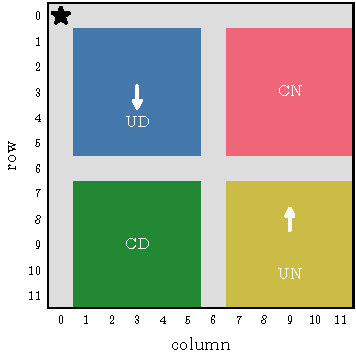
\includegraphics{fig_e1_env.pdf}
  \caption{The E1 environment (a torus): corridor (grey), goal (star) and the four blocks with their dynamics type;
    arrows: the drift of the two uncontrollable blocks for the retained direction, away from the goal.}
  \label{fig:env}
\end{figure}

\paragraph{What is sought.}
Overall, this part looks at how accurately our theoretical values are recovered, and how precisely depending on the
amount of data used.
No phenomenon is expected here: in the tabular setting the transition probabilities of a state live independently of
those of the other states, so no propagation or generalisation is possible in this version; if we saw one, it would be a
bug.

\paragraph{Data and estimation.}
E1 collects its data with a generative model, with no policy at all: $n$ is fixed (10, 30, 100, 300 or 1000) and $n$ % num-ok
% src: experiments/E1_offline_4zones/run_etape_b.py (BUDGETS: a code constant, no config key)
transitions are drawn independently for each pair (state, action); the notion of trajectory does not exist here.
The collected data are not influenced by the belief, so no belief/exploration loop is possible: it is the ideal,
cleanest setting for our floor.
The tensor of transition probabilities, $\That$, is estimated by counting, and our measures are made from these
probability distributions, over \eOneNSeeds{} seeds.
The same is done in a control environment, identical except that each uncontrollable zone is replaced by its
controllable version with the same noise level: it is the one that gives $\Iref$.

\paragraph{Measures.}
Our measures are $\Ihat(s)$; $\Ihat(\text{zone})$, the mean of $\Ihat(s)$ over the zone; $\bhat(s) = \Ihat(s) - \Iref(s)$;
and $\regret(s) = \Vstar(s) - V^{\pi}(s)$, the value actually lost in the true world by the policy $\pi$ derived from the
estimated model, compared with the optimal policy.
$\Ihat$, $\bhat$ and $\Lone$ are averaged over the \eOneZoneCells{} cells of the zone, whereas $\regret$ is averaged
over the interior cells only, that is, those whose four neighbours are in the zone (the central $3 \times 3$ square, % num-ok
\eOneInteriorCells{} cells, with the same geometric definition for every zone type).
The reason is that $\Ihat$, $\bhat$ and $\Lone$ are local: they depend only on the transition row of the cell, which is the
same everywhere in the zone, so all cells are kept for precision. $\regret$ goes through the value, which is not local:
a boundary cell is one step from the exit, and its value is largely set by what lies on the other side, so averaging it
with the others would mix the effect of the zone with the effect of its neighbour. The interior carries the comparison
between zones, the boundary is reported separately as a description, and since each mean of $\regret$ rests on only
\eOneInteriorCells{} values, this count is shown next to it.
Note that we must find $\regret(s) \geq 0$ for every $s$. % num-ok
% src: experiments/E1_offline_4zones/report.py (PRECISION_TOL: a code constant, no config key)
The tolerance fixed in advance: $\bhat$ must fall within 0.03 bit of its theoretical value. % num-ok

% =====================================================================================================================
\section{Step A: $\gamma$, $\Rgoal$ and the drift direction}
\label{sec:stepA}
% src: notes

Before measuring anything, three parameters that set what uncontrollability costs had to be fixed: $\gamma$, the reward
$\Rgoal$ at the goal, and the direction of the drift in the uncontrollable zones (toward the goal or away from it).
No learning is needed for that; it is Step~A: $\Vstar$ is computed by value iteration under the true kernel, in the
environment and in its control, for \eOneCalibCombos{} combinations (\eOneCalibGammas{} values of $\gamma$
$\times$ \eOneCalibRewards{} of $\Rgoal$ $\times$ \eOneCalibDirections{} directions); in short, dynamic programming with
a perfect model.

\paragraph{The flat exterior.}
We initially expected an uncontrollable zone to dig a well of value that would spill over its neighbourhood, and had
planned two tools for it: a curve of $\Vstar$ outside the zones as a function of the distance to each uncontrollable
zone, and a regression to check that the wells of the two zones stayed separable (which was to constrain $\gamma$, a
too large $\gamma$ propagating value too far).
Instead, we found that the exterior is flat: outside the uncontrollable zones, $\Vstar$ is the same in the environment
and in the control up to at most \eOneExteriorDiffCtrl{} over the \eOneCalibCombos{} combinations, and the same between
the two drift directions up to at most \eOneExteriorDiffDirection.
The reason is simple: the corridor gives every exterior cell a shortest path to the goal that is entirely controllable
and never crosses an uncontrollable zone, so an optimal agent never sets foot there and the nature of these zones changes
nothing for it.
Inside the zones, by contrast, the gap with the control reaches \eOneInteriorGapMax.
This is our flat null model: under perfect planning, uncontrollability produces no spatial gradient outside.

\paragraph{Three reading errors.}
Along the way, three reading errors were corrected (the code was right, the interpretation was wrong).
1) The curve was not a well (Figure~\ref{fig:exterior}): it decreases with the distance to the zone, so the value is % num-ok
higher near the zone, the wrong direction for a well; it is only that the goal touches the corner of the blocks, so
``near the zone'' means ``near the goal'': it is a distance-to-goal profile.
% src: experiments/E1_offline_4zones/artifacts/gradient_curves.csv
2) The curves ``distance to the north-west zone'' and ``distance to the south-east zone'' are identical to machine % num-ok
precision (largest difference \eOneProfileDiffNWSE): they were not two independent measurements but a single one, and one
more confirmation that the exterior does not tell the zones apart.
3) The separability regression was computed in the control environment, where no zone is uncontrollable, so its result % num-ok
near zero was mechanical, and it had wrongly been counted among the criteria that passed; it is moot, since there are no
exterior wells to separate.

% src: experiments/E1_offline_4zones/artifacts/gradient_curves.csv
\begin{figure}[t]
  \centering
  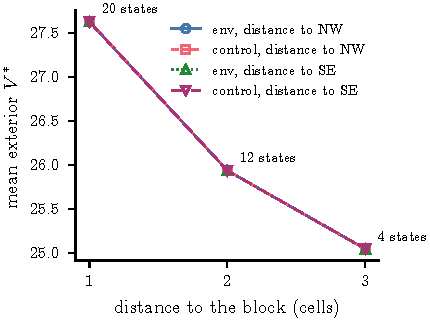
\includegraphics{fig_e1_exterior.pdf}
  \caption{Step A, at the frozen $\gamma$, $\Rgoal$ and drift direction: mean $\Vstar$ of the exterior states against the
    distance to each uncontrollable block, in the environment and in its control. The four curves coincide; the number
    of states per distance bin is annotated.}
  \label{fig:exterior}
\end{figure}

\paragraph{The choices.}
The retained drift direction is away from the goal, without ambiguity (Figure~\ref{fig:calibration}).
With a drift toward the goal, the gap is zero in the deterministic zone in \eOneTowardNegligible{} of the
\eOneCalibPerDirection{} combinations (the drift coincides with the optimal action, so controlling nothing costs
nothing), whereas with the opposite drift there is a real interior well in both zones in \eOneAwayWells{} of the
\eOneCalibPerDirection.
Note that the control always does at least as well as the environment (having the choice cannot hurt), so the gap can
only be negative or zero.
For $\gamma$ and $\Rgoal$, the initial constraint (separating the wells) having disappeared, we chose
$\gamma = \eOneGamma$ and $\Rgoal = \eOneGoalReward$ on three criteria: the interior well is deepest at
$\gamma = \eOneGamma$; at $\Rgoal = \eOneGoalReward$ the value inside the uncontrollable zones stays positive (a zone of
negative value would be a trap to flee, not an uncontrollable zone, and that would distort E2); and the accumulated cost
of the steps, $1/(1-\gamma) = \eOneStepCostHorizon$, is \eOneStepCostShare\,\% of $\Rgoal$, so it really counts. % num-ok
These three values are frozen; they are where the $\gamma = \eOneGamma$ and the $+$\eOneGoalReward/\eOneStepReward{} of E2
and E3 come from.

% src: experiments/E1_offline_4zones/artifacts/calibration_report.csv
\begin{figure}[t]
  \centering
  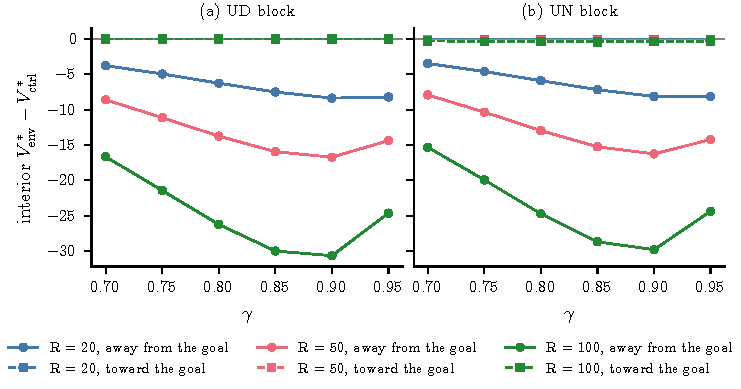
\includegraphics{fig_e1_calibration.pdf}
  \caption{Step A: the interior gap $\Vstar_{\mathrm{env}} - \Vstar_{\mathrm{ctrl}}$ inside each uncontrollable block
    against $\gamma$, for each $\Rgoal$ and both drift directions (perfect model).}
  \label{fig:calibration}
\end{figure}

\paragraph{Scope.}
An important limit: the flat null model holds only for a perfect model.
As soon as the model is learned, hence wrong, planning on it can propagate estimation errors from a cell to its
neighbours and create a structure that depends on the distance without any belief having generalised; E1 does not cover
this mechanism, it is E2's job.
Consequences for what follows: in E4, with a model close to the true one, any behavioural gradient observed outside the
uncontrollable zones will be attributable to the belief and not to the propagation of value;
\todo{E4 is not described in this report: a sentence on what E4 tests would make this consequence readable.}
and in E2/E3, a zero $\regret$ outside the zones is the expected result.

% =====================================================================================================================
\section{Step B: protocol}
\label{sec:stepB}
% src: notes

We then move to Step~B, the validation proper.
The protocol: for each $n$ in $\{10, 30, 100, 300, 1000\}$, exactly $n$ transitions are drawn per pair $(s, a)$ with the % num-ok
generative model, in the environment and in its control, over \eOneNSeeds{} seeds.
$\That$ is estimated by plain counting (the observed frequencies), which is legitimate here since every pair necessarily
has data.
% src: experiments/E1_offline_4zones/run_etape_b.py (alpha=0.0 only); experiments/E1_offline_4zones/estimation.py
A variant with a Dirichlet prior restricted to the 5 possible successors is implemented and unit-tested, but it is % num-ok
absent from the delivered grid and has no result; it is the estimator that serves in E2.
For $\regret$, the policy is obtained by planning on $\That$; the planner's values are then discarded and this policy is
evaluated again under the true kernel, never under $\That$.

% =====================================================================================================================
\section{Step B: accuracy, bias cancellation, deciding against modelling}
\label{sec:results}
% src: notes

\paragraph{First result: accuracy.}
$\bhat$ recovers the theory in every zone at $n = 1000$ (mean $\pm$ standard deviation over \eOneNSeeds{} seeds, whole % num-ok
zone; Figure~\ref{fig:b}a).
Conveyor belt: $\eOneBUDMean \pm \eOneBUDSd$, that is $-\logtwo \eOneNActions$ exactly.
Uncontrollable-noisy: $\eOneBUNMean \pm \eOneBUNSd$ for \eOnePredBUN{} predicted, an error of \eOneBUNError, far below
the tolerance of 0.03 bit. % num-ok
Controllable-noisy: $\eOneBCNMean \pm \eOneBCNSd$, so 0. % num-ok
Controllable-deterministic: exactly \eOneBCDMean.
In both deterministic zones, $\Ihat$ is exact from $n = 10$, which is normal: a deterministic transition is known % num-ok
perfectly from the first draw.
And $\regret \geq 0$ holds without any violation (\eOneDeltaViolations) over the \eOneNRows{} measurement rows. % num-ok

\paragraph{Second result: the estimation bias cancels in $\bhat$.}
This is the result that justifies the whole paired design.
With few data, $\Ihat$ is biased upward (sampling chance makes the actions look like actions that have an effect).
In the uncontrollable-noisy zone at $n = 10$, the bias of $\Ihat$ is \eOneBiasIhat{} bit and that of its reference % num-ok
\eOneBiasIref{} bit, but the error that remains in $\bhat$ is only \eOneBiasResidual{} bit, a cancellation factor of about
\eOneBiasFactor{} (Figure~\ref{fig:b}b).
It works because the environment and its control have, by construction, the same support and the same conditional
entropy, so both sides err almost alike and the error goes away in the subtraction.
This is exactly the argument reused in E3 to hope that $\bhat$ cancels the bias of hybrid codes.

% src: experiments/E1_offline_4zones/artifacts/measurements.csv
\begin{figure}[t]
  \centering
  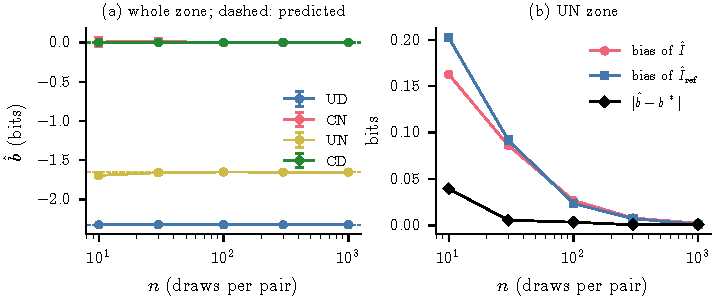
\includegraphics{fig_e1_b_vs_n.pdf}
  \caption{(a) $\bhat$ by zone against the number of draws per pair, whole zone, mean $\pm$ standard deviation over
    \eOneNSeeds{} seeds; dashed lines: predicted values. (b) Uncontrollable-noisy zone, whole zone: the bias of $\Ihat$
    in the environment and of $\Iref$ in its control, and the error left in $\bhat$.}
  \label{fig:b}
\end{figure}

\paragraph{Third result: deciding well needs fewer data than modelling well.}
\todo{Define $\Lone$ (the error of $\That$ against $P$) at its first use.}
In the controllable-noisy zone, $\regret$ (interior states) goes from \eOneDeltaCNTen{} ($n = 10$) to \eOneDeltaCNThirty, % num-ok
\eOneDeltaCNHundred, \eOneDeltaCNThreeHundred{} and then \eOneDeltaCNThousand{} at $n = 1000$, while $\Lone$ (whole % num-ok
zone) goes from \eOneLoneCNTen{} to \eOneLoneCNThousand{} (Figure~\ref{fig:delta}).
In the uncontrollable-noisy zone, $\regret$ falls to 0 from $n = \eOneDeltaUNZeroAt$, while $\Lone$ is still % num-ok
\eOneLoneUNAtZero, \eOneLoneUNRatio{} times its final value: the policy is already the right one while the model is still
far from having converged.

Two reading pitfalls were avoided.
First, $\regret$ and $\Lone$ are not in the same unit ($\regret$ is a value, up to \eOneGoalReward; $\Lone$ a probability
% src: notes (the bound of L1)
mass, bounded by 2), so we never speak of a ``crossing'' of their curves: it would depend on the scale of $\Rgoal$. % num-ok
Second, in both deterministic zones $\regret$ is 0 at every budget, but this is trivial (the transition is exact from one % num-ok
draw); it is not a finding about the task.

% src: experiments/E1_offline_4zones/artifacts/measurements.csv
\begin{figure}[t]
  \centering
  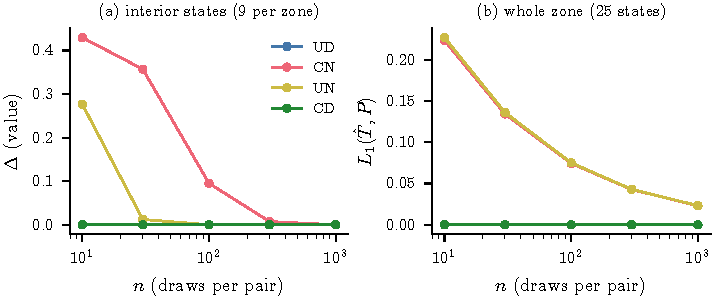
\includegraphics{fig_e1_delta_l1.pdf}
  \caption{(a) $\regret$ by zone against the number of draws per pair: mean over \eOneNSeeds{} seeds of the zone's
    interior states (\eOneInteriorCells{} per zone). (b) $\Lone$ error of $\That$ by zone, whole zone
    (\eOneZoneCells{} states). Separate axes: $\regret$ is a value, $\Lone$ a probability mass.}
  \label{fig:delta}
\end{figure}

% =====================================================================================================================
\section{Detectability}
\label{sec:detectability}
% src: notes

E1's main deliverable is detectability: the smallest $|\bhat|$ that can be told apart from zero, as a function of $n$.
It is measured in the controllable zones, because that is where the null hypothesis $\bhat = 0$ is really true (the same % num-ok
dynamics in the environment and in the control).

\paragraph{Two null models.}
There are two null models, which do not answer the same question.
% src: experiments/E1_offline_4zones/run_etape_b.py (N_PERMUTATIONS: a code constant, no config key)
The first is a permutation test: in a zone, the action labels of all the (action, successor) draws are shuffled, 500 % num-ok
times, and $\Ihat$ is recomputed each time. This breaks any link between action and outcome, so it tests
$\Hnull{}: I = 0$, ``is $\Ihat$ distinguishable from zero'', and it is an exact test conditionally on the observed % num-ok
counts. It is applied only to the zone-aggregated $\Ihat$, never state by state.
The second is a bootstrap: datasets are redrawn from the observed distributions, action by action, and we look at the
distribution of $\bhat$ we would obtain with fresh data. It measures the precision of the estimator around its true value,
and it is the one used for detectability.
The threshold reported is the 95th percentile of $|\bhat|$ under this null, averaged over the seeds. % num-ok
A small difference between the two nulls is normal, since they do not ask the same question; it is not a sign that one is
wrong.

\paragraph{Results.}
In the controllable-noisy zone, the detectable threshold goes from \eOneThresholdTen{} bit ($n = 10$) to % num-ok
\eOneThresholdThirty{} ($n = 30$), \eOneThresholdHundred{} ($n = 100$), \eOneThresholdThreeHundred{} ($n = 300$) and % num-ok
\eOneThresholdThousand{} ($n = 1000$) (Figure~\ref{fig:detectability}). % num-ok
The $\bhat$ actually observed in this zone is small and non-zero, as expected: its standard deviation between seeds goes
from \eOneBSdCNTen{} at $n = 10$ down to \eOneBSdCNThousand{} at $n = 1000$. % num-ok
In the controllable-deterministic zone the threshold is exactly \eOneThresholdCD{} at every budget (no estimation noise on
a deterministic transition): a degenerate case, reported separately and never averaged with the noisy zone.
And in the uncontrollable zones this null has no meaning for detectability, since $\bhat$ is really different from zero
there (\eOnePredBUD{} and \eOnePredBUNShort): the numbers are kept for the record but labelled as the wrong number to cite.

\paragraph{An anomaly.}
Ordinary sampling noise decreases as $1/\sqrt{n}$, so in log-log the slope of the threshold should be $-0.5$. % num-ok
We find \eOneSlope, with a 95\,\% interval of [\eOneSlopeLow, \eOneSlopeHigh]: $-0.5$ is outside, and since each point % num-ok
already averages \eOneNSeeds{} seeds, it is a real difference, not noise.
A first explanation (a residual contamination in $1/n$) was put forward and then retracted because it had the wrong % num-ok
sign: a term in $1/n$ decreases faster than $1/\sqrt{n}$, so it would make the slope steeper, not shallower. % num-ok
Three candidates were then tested.
1) The point $n = 10$ would lie outside the asymptotic regime (and it weighs most in a log-log fit): without it the % num-ok
slope becomes \eOneSlopeNoTen{} [\eOneSlopeNoTenLow; \eOneSlopeNoTenHigh], which explains about a third of the gap, but
$-0.5$ stays outside. % num-ok
% src: experiments/E1_offline_4zones/README.md (500 vs 5000; per-state slopes on 5 seeds: -0.407, aggregate -0.408)
2) A bias in the estimate of the percentile itself, due to only 500 draws: tested with 500 against 5000 draws, no % num-ok
difference beyond noise; ruled out.
3) An aggregation artefact, states that would each follow $-0.5$ but with different amplitudes: ruled out too. The % num-ok
per-state slopes, computed with 5 seeds averaged, are $-0.407$ on average and none reaches $-0.5$, and the aggregate % num-ok
slope computed the same way ($-0.408$) equals their mean, so the shallow slope is a property of each state, not an % num-ok
effect of averaging.
Outcome: partly explained by $n = 10$, the rest unresolved; it is written as such rather than inventing an unverified % num-ok
mechanism.

% src: experiments/E1_offline_4zones/artifacts/permutation_null.csv
\begin{figure}[t]
  \centering
  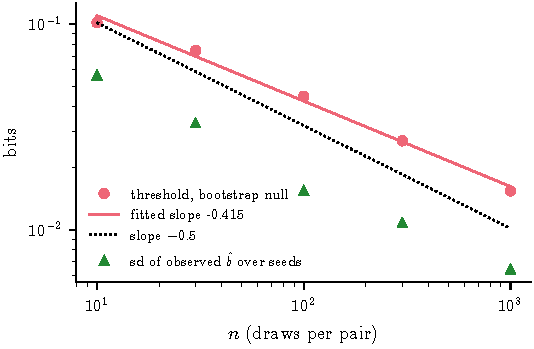
\includegraphics{fig_e1_detectability.pdf}
  \caption{Detectability in the controllable-noisy zone (whole zone): the threshold (95th percentile of $|\bhat|$ under % num-ok
    the bootstrap null, mean over \eOneNSeeds{} seeds) against the number of draws per pair, with its fitted power law,
    a slope $-0.5$ reference, and the standard deviation of the observed $\bhat$ over the seeds.} % num-ok
  \label{fig:detectability}
\end{figure}

\paragraph{Two benchmarks for what follows.}
The effect of \eTwoEffectCN{} bit that we will find in E2 in the controllable-noisy zone is detectable only from the
order of $n = 1000$ visits per pair (threshold \eOneThresholdThousand); and it is this same order of magnitude, a few % num-ok
hundredths of a bit, that serves as the yardstick to judge the resolution of E3.

% =====================================================================================================================
\section{Bugs, corrections and checks}
\label{sec:bugs}
% src: notes

Three real bugs were found and fixed during Step~B, each locked afterwards by a regression test.

\paragraph{1) Seeds correlated between the environment and the control.} % num-ok
The two collections meant to be independent each created their own generator, but with the same integer, so the two
generators produced exactly the same sequence of numbers.
In a controllable zone, the environment and the control have the same kernel, so the same probabilities and the same
random numbers give the same draws: $\bhat$ was exactly 0 with zero variance in both controllable zones. % num-ok
It was true by construction, not by measurement, and as a result no detectability threshold had ever been computed where
$\bhat = 0$ is really true. % num-ok
The warning sign is the zero variance: a measurement made on noisy data that falls exactly on zero is suspicious.
It was fixed by deriving independent streams with \texttt{SeedSequence.spawn}, and a shared-seed test was deliberately
kept, which checks that the control is identical to the environment in a controllable zone (the bug recycled as a test).
This is the seeding scheme reused in E2 and E3.

\paragraph{2) The bootstrap pooled the actions before resampling.} % num-ok
This is correct to test $I = 0$, but wrong for the detectability of $\bhat$ in a controllable zone: pooling erases the true % num-ok
dependence between action and outcome, and the statistic then behaves like that of an independence test, which decreases
as $1/n$, instead of an estimation noise around a true non-zero value, which decreases as $1/\sqrt{n}$. % num-ok
It was seen empirically (a threshold falling as $1/n$, too fast to be honest) before being understood. % num-ok
It was fixed by resampling each action from its own observed distribution, with a test that requires the threshold to
decrease more slowly than $1/n$. % num-ok

\paragraph{3) A retracted claim.} % num-ok
We had written that the permutation test was ``too narrow'' and that the bootstrap corrected it. This is false: a
permutation test conditional on the observed counts is exact by construction. The two nulls simply answer different
questions.

\paragraph{The recommendation of $n$, corrected twice.}
% src: experiments/E1_offline_4zones/README.md (relative error of an sd: about 35 % with 5 seeds, 16 % with 20)
First correction: with 5 seeds, a standard deviation is estimated to within about 35\,\%, so what was read as a plateau % num-ok
or a non-monotonicity of the precision was only estimation noise.
We moved to \eOneNSeeds{} seeds (about 16\,\%) and replaced the point-by-point reading by a fit of a $1/\sqrt{n}$ curve % num-ok
on all budgets at once.
% src: experiments/E1_offline_4zones/README.md (the fitted curve's raw crossing near n = 17)
Second correction: the first recommendation was $n = 30$: the fitted curve crosses the tolerance of 0.03 bit near % num-ok
$n \approx 17$, and 30 is the smallest budget tested beyond that crossing. % num-ok
But this crossing is where the error of a typical run equals the tolerance, not where it is reliably met: counted
directly, \eOneOutOfTolThirty{} seeds out of \eOneNSeeds{} (\eOneOutOfTolThirtyShare\,\%) exceeded 0.03 bit at % num-ok
$n = 30$ in the uncontrollable-noisy zone. % num-ok
The right criterion is the curve plus a safety margin of $k$ standard deviations, which multiplies $n$ by $k^2$ since the % num-ok
standard deviation decreases as $1/\sqrt{n}$ (Figure~\ref{fig:precision}). % num-ok
At 2 sigma the crossing falls near \eOneCrossingTwoSigma, hence $n = \eOneRecommendedN$ (\eOneOutOfTolRecommended{} % num-ok
seeds out of \eOneNSeeds{} out of tolerance, checked); at 3 sigma near \eOneCrossingThreeSigma, hence % num-ok
$n = \eOneRecommendedNThree$.
Recommendation retained: $n = \eOneRecommendedN$ visits per pair for E2/E3, with the reservation that it is a precision
recommendation established on the zones with a known effect, to be confronted with detectability in the controllable
zones.

% src: experiments/E1_offline_4zones/artifacts/measurements.csv
\begin{figure}[t]
  \centering
  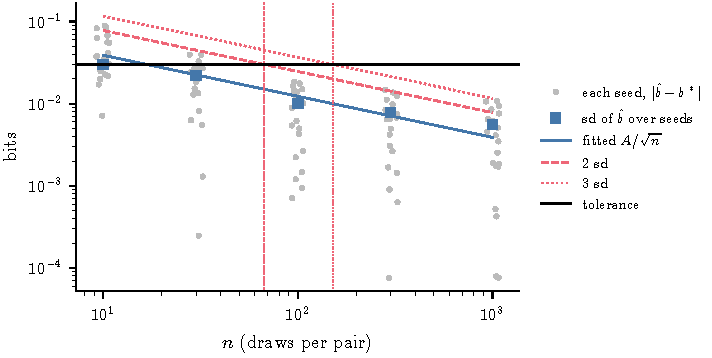
\includegraphics{fig_e1_precision.pdf}
  \caption{The recommended $n$, uncontrollable-noisy zone (whole zone): each seed's error $|\bhat - b^*|$, the standard
    deviation of $\bhat$ over the seeds, the fitted $A/\sqrt{n}$ curve and its 2- and 3-sigma versions against the % num-ok
    tolerance; vertical lines: the fitted crossings.}
  \label{fig:precision}
\end{figure}

\paragraph{Performance and a trial run.}
% src: experiments/E1_offline_4zones/README.md (more than 60 min; a trial run of about one minute, 1 seed)
On the performance side, the first corrected version of the null computation was unusable (more than an hour without
finishing) because it drew the samples one by one; we moved to a vectorised multinomial draw, whose equivalence was
checked statistically by a chi-squared test (not sample by sample, which is impossible since the two versions do not
consume the generator in the same way).
And before launching the full grid, a trial run of one minute on one seed checked three things: $\bhat$ non-zero in the
controllable-noisy zone, $\regret \geq 0$ everywhere, and a detectability slope in the right direction. % num-ok

% =====================================================================================================================
\section{What E1 hands on}
\label{sec:legacy}
% src: notes

$\gamma = \eOneGamma$, $\Rgoal = \eOneGoalReward$ and the drift away from the goal; the tolerance of 0.03 bit; % num-ok
$n = \eOneRecommendedN$; the scheme of independent seeds; the pairing of environment and control, and the proof that it
cancels the bias; and the methodological lesson that the three bugs were caught by shape tests (a zero variance, a slope
that was too steep) and not by checking whether the values looked plausible.

\bibliographystyle{plainnat}
\bibliography{../refs}

\end{document}
